\subsection{Concurrency in the Linux Kernel}
\label{concurrency}

Nowadays, multicore architectures have become the mainstream, leading to an ever-increasing demand for concurrency in operating systems. For example, modern Linux kernel distributions address this demand by providing multiple sources of concurrency~\cite{corbet2005linux}: the kernel can invoke an arbitrary number of entry points from the same driver concurrently to perform device related operations; a running driver process can block and be replaced by another process in the same driver; hardware interrupts can be handled concurrently; delayed code execution is the norm; and the user can insert or remove hardware components without rebooting the kernel (known as hot-plugging). All these possibilities can easily lead to serious concurrency issues, such as \emph{data races}, which can be defined as follows:

\begin{definition}
\label{definition:datarace}
A data race occurs when two distinct threads access a shared memory location, at least one of the accesses modifies the location, and there is no mechanism in place to prevent these accesses from being simultaneous.
\end{definition}

Listing~\ref{data_race_example} is an example of a data race between two entry points of a Linux driver. The resource \texttt{dev->resource} is shared between the two entry points \texttt{ep1} and \texttt{ep2}. Entry point \texttt{ep1} writes the value 5 to \texttt{dev->resource}, and entry point \texttt{ep2} writes the value 3 to \texttt{dev->resource} if the value of \texttt{dev->resource} is not 5. A data race can occur if \texttt{ep1} and \texttt{ep2} run concurrently: the read and write accesses to the shared resource may execute in arbitrary order leading to nondeterministic behaviour.

%\begin{figure}[!h]
%\centering
%\noindent\begin{minipage}{.95\textwidth}
%\noindent\begin{minipage}{.485\textwidth}
%\begin{lstlisting}[caption={Example of a simple data race in a Linux device driver.},
%label=data_race_example]
%static void ep1 (struct shared *dev) {
%  dev->resource = 5;
%}
%
%static void ep2 (struct shared *dev) {
%  if (dev->resource != 5)
%    dev->resource = 3;
%}
%\end{lstlisting}
%\end{minipage}\hfill
%\noindent\begin{minipage}{.485\textwidth}
%\begin{lstlisting}[caption={Data race eliminated by using the highlighted locks.},
%label=lock_example]
%static void ep1 (struct shared *dev) {
%@lock(&dev->lock);@
%  dev->resource = 5;
%@unlock(&dev->lock);@
%}
%
%static void ep2 (struct shared *dev) {
%@lock(&dev->lock);@
%  if (dev->resource != 5)
%    dev->resource = 3;
%@unlock(&dev->lock);@
%}
%\end{lstlisting}
%\end{minipage}
%\end{minipage}
%\end{figure}

The most common technique for eliminating data races is using a \emph{locking} mechanism. Locking a set of program statements that access a shared resource creates a \emph{critical section}, i.e. source code that cannot be executed by more than one thread simultaneously. Listing~\ref{lock_example} shows how to use a lock to eliminate the data race in the previous example.

Lock-based synchronisation is a powerful tool for preventing data races in drivers, but careless use of locks has multiple pitfalls~\cite{sutter2005software}. Coarse-grained locking can severely hurt performance, because it limits the opportunity for concurrency. On the other hand, fine-grained locking can easily lead to \emph{deadlocks}, a system-halting situation in which no active thread can progress, because it is waiting to acquire a lock that is held by another blocked thread. Although the Linux kernel provides sophisticated lock-free synchronisation mechanisms~\cite{corbet2005linux}, in this work we choose to focus on reasoning about locks.

\subsection{Limitations in Reasoning about Thread Interleavings}

A fundamental concept in concurrency analysis is Lamport's \emph{happens-before} relation~\cite{lamport1978time}, which denotes a partial-order between all events during a concurrent execution of a program. The happens-before relation can be defined as follows:

\begin{definition}
\label{definition:datarace}
Let $E_1$ and $E_2$ be two events during a program's concurrent execution. If $E_1$ and $E_2$ are in the same thread and $E_1$ occurs before $E_2$, or if $E_1$ and $E_2$ are in different threads and there is a synchronisation mechanism that prevents a thread schedule in which $E_2$ occurs before $E_1$, then $E_1 \rightarrow E_2$, where the symbol $\rightarrow$ denotes the happens-before relation.
\end{definition}

Happens-before is transitive, i.e. for any three events $E_1$, $E_2$ and $E_3$, if $E_1 \rightarrow E_2$ and $E_2 \rightarrow E_3$, then $E_1 \rightarrow E_3$. If two events $E_1$ and $E_2$ occur in different threads, and neither $E_1 \rightarrow E_2$, nor $E_2 \rightarrow E_1$ holds, then $E_1$ and $E_2$ happen concurrently, which indicates a data race if the two events access the same shared resource and at least one of the accesses is a modifier. Figure~\ref{happens_before} shows an example of applying happens-before reasoning in two concurrently running entry points of a driver. Each of the three statements \{A, B, C\} in thread 1 is executed before the next one, and thus all of them are ordered by the happens-before relation. The same applies for each of the four statements \{D, E, F, G\} in thread 2. Statement C in thread 1 releases the lock, and subsequently allows D in thread 2 to acquire the same lock. Thus, $C \rightarrow D$. This means that for this specific thread interleaving the set of statements \{A, B, C\} happens before the set of statements \{D, E, F, G\}.

\begin{figure}[htbp]
\centering
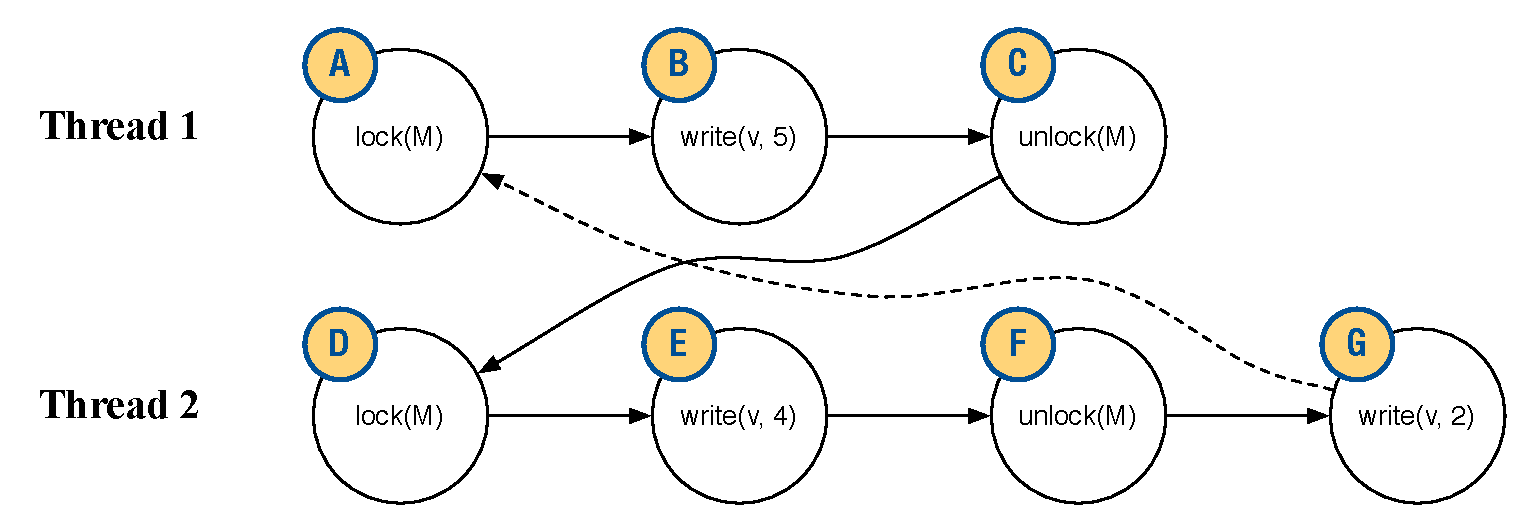
\includegraphics[width=.95\linewidth]{img/happens_before.pdf}
\caption{Example showcasing the main limitation of happens-before.}
\label{happens_before}
\end{figure}

The above example showcases the main limitation of happens-before. If the technique explores \emph{only} this specific thread interleaving, it will miss a potential data race between statements B and G, because $B \rightarrow G$ in this specific schedule. Thus, a tool based on happens-before requires a scheduler that produces as many different thread interleavings as possible to increase execution path coverage~\cite{savage1997eraser}. Achieving full coverage with tools based on happens-before is infeasible though, because of the exponential number of possible thread interleavings in realistic concurrent programs. Furthermore, attempting to explore a large number of thread schedules quickly leads to scalability issues~\cite{musuvathi2008finding}. Thus, previous work based on happens-before typically explore paths under a certain bound, such as the number of allowed context switches~\cite{qadeer2004kiss}.